\documentclass[a4paper,12pt]{article} 
% Paquetes......................................................................
\usepackage{amsmath, amssymb, amsfonts, latexsym}
\usepackage[utf8]{inputenc}
\usepackage{palatino}
\usepackage{pdfpages}
\usepackage{float} % para que las figuras no floten

\renewcommand{\contentsname}{Contenidos}

\textheight = 24 cm
\textwidth = 17 cm

%\renewcommand{\arraystretch}{1.25}

% INICIO DEL DOCUMENTO --------------------------------------------------------
\begin{document}
	
	\setlength{\parindent}{0.5cm}
	\setlength{\voffset}{-2cm}
	\setlength{\hoffset}{-2cm}
	
	%%%%%%%%%%%%%%%%%%%%%%%%%%%%%%%%%%%%%%%%%
% Academic Title Page
% LaTeX Template
% Version 2.0 (17/7/17)
%
% This template was downloaded from:
% http://www.LaTeXTemplates.com
%
% Original author:
% WikiBooks (LaTeX - Title Creation) with modifications by:
% Vel (vel@latextemplates.com)
%
% License:
% CC BY-NC-SA 3.0 (http://creativecommons.org/licenses/by-nc-sa/3.0/)
% 
% Instructions for using this template:
% This title page is capable of being compiled as is. This is not useful for 
% including it in another document. To do this, you have two options: 
%
% 1) Copy/paste everything between \begin{document} and \end{document} 
% starting at \begin{titlepage} and paste this into another LaTeX file where you 
% want your title page.
% OR
% 2) Remove everything outside the \begin{titlepage} and \end{titlepage}, rename
% this file and move it to the same directory as the LaTeX file you wish to add it to. 
% Then add \input{./<new filename>.tex} to your LaTeX file where you want your
% title page.
%
%%%%%%%%%%%%%%%%%%%%%%%%%%%%%%%%%%%%%%%%%

%----------------------------------------------------------------------------------------
%	PACKAGES AND OTHER DOCUMENT CONFIGURATIONS
%----------------------------------------------------------------------------------------


%----------------------------------------------------------------------------------------
%	TITLE PAGE
%----------------------------------------------------------------------------------------

\begin{titlepage} % Suppresses displaying the page number on the title page and the subsequent page counts as page 1
	\newcommand{\HRule}{\rule{\linewidth}{0.5mm}} % Defines a new command for horizontal lines, change thickness here
	
	\center % Centre everything on the page
	
	%------------------------------------------------
	%	Headings
	%-----------------------------------------s-------
	
	\textsc{\Large Máster en Inteligencia Artificial}\\[1.5cm] % Main heading such as the name of your university/college
	
	\textsc{\LARGE Informática Biomédica}\\[0.5cm] % Major heading such as course name
	
	%\textsc{\large Minor Heading}\\[0.5cm] % Minor heading such as course title
	
	%------------------------------------------------
	%	Title
	%------------------------------------------------
	
	\HRule\\[0.4cm]
	
	{\huge\bfseries Buscador de LOINC con BM25\\\vspace{1.5mm}
		 optimizado usando clicks de usuarios*}\\[0.4cm] % Title of your document
	%LOINC search engine using clickthrough data
	\HRule\\[1.2cm]
	
	%------------------------------------------------
	%	Author(s)
	%------------------------------------------------
	
	%\begin{minipage}{0.4\textwidth}
	%	\begin{flushleft}
	%		\large
	%		\textit{Author}\\
	%		\textsc{Aída Muñoz Monjas} % Your name
	%	\end{flushleft}
	%\end{minipage}
	%~
	%\begin{minipage}{0.4\textwidth}
	%	\begin{flushright}
	%		\large
	%		\textit{Supervisor}\\
	%		Dr. Caroline \textsc{Becker} % Supervisor's name
	%	\end{flushright}
	%\end{minipage}
	
	% If you don't want a supervisor, uncomment the two lines below and comment the code above
	{\Large\textit{Autores}}\\
	
	{\large\textsc{
			 Aída Muñoz Monjas\\
			 Gabriel Rivera Cárdenas\\
			 César Pantoja Rosales} } % Your name
	
	%------------------------------------------------
	%	Date
	%------------------------------------------------
	
	\vfill\vfill\vfill % Position the date 3/4 down the remaining page
	
	{\large\today} % Date, change the \today to a set date if you want to be precise
	
	%------------------------------------------------
	%	Logo
	%------------------------------------------------
	
	%\vfill\vfill
	%\includegraphics[width=0.2\textwidth]{placeholder.jpg}\\[1cm] % Include a department/university logo - this will require the graphicx package
	 
	%----------------------------------------------------------------------------------------
	
	\vfill % Push the date up 1/4 of the remaining page
	
\end{titlepage}

%----------------------------------------------------------------------------------------

%\end{document}

	
	%\tableofcontents

	
	\section{Introducción}
	Tradicionalmente, algoritmos como el TF-IDF usados para realizar motores de búsqueda clasifican los resultados obtenidos para cada consulta en "relevantes" e "irrelevantes". Esta clasificación no caracteriza de manera completamente correcta las opiniones de los usuarios, ya que hay resultados más relevantes que otros, de manera que se puede establecer un orden prácticamente total de la relevancia óptima de los resultados.
	
	Obtener este ranking sin tener un feedback explícito no es trivial, y conseguir estos comentarios por parte de los usuarios es difícil. El conocimiento sobre a qué entradas de la búsqueda acceden los usuarios nos puede proporcionar información equivalente, de manera mucho menos costosa. El principal inconveniente de utilizar el conocido como "clickthrough data", datos sobre los clicks de los usuarios, es la cantidad de ruido presente en los datos y la dependencia que existe entre los clicks de los usuarios y el orden de los documentos recibidos.
	
	Sin duda este tipo de datos son útiles y poco costosos de conseguir, pero su calidad no se puede comparar con la de juicios de relevancia generados por expertos del dominio.\\
	
	En este trabajo, se nos pide implementar los algoritmos descritos en el artículo \cite{articulo-clase} sobre un set de tres búsquedas sobre la terminología LOINC.
	
	LOINC (Logical Observation Identifiers, Names and Codes)\cite{loinc} es una terminología de términos de laboratorio, donde cada concepto viene definido por el componente medido (component), el sistema sobre el que se observa (system), la propiedad observada (property) y su nombre (long common name), este último agrupando las otras tres características del término.
	
	\section{Desarrollo del buscador}
	Utilizando el lenguaje python, se ha adaptado el dataset proporcionado a las necesidades del proyecto, y se ha preparado una implementación de un buscador basado en el algoritmo BM25, optimizado mediante los clicks de los usuarios.
	
	\subsection{Procesado de datos y aplicación del BM25}
	
	En el dataset se proporcionaron tres búsquedas sobre LOINC, de las cuales cada consulta tenía una lista de posibles respuestas.
	Para cada una de las consultas se obtuvo un dataset similar al de la Figura 1.
	%, donde cada una de las columnas contiene información importante sobre cada una de las posibles salidas de la búsqueda.
	
	 \begin{figure}[H]
	 	\centering
	 	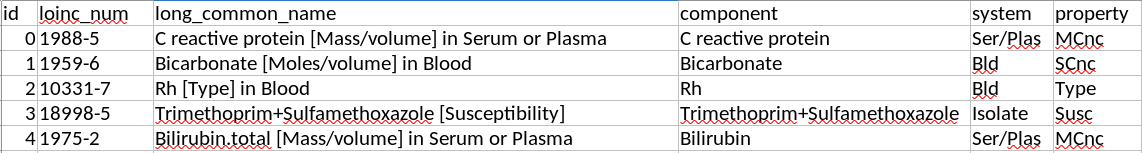
\includegraphics[width=\textwidth]{include/query_example_orig.png}
	 	\caption{Ejemplo del dataset recibido para la consulta "glucose in blood"}
	 \end{figure}
	
	El procesado de los datos de este problema se ve afectado por dos importantes decisiones de diseño: la elección del algoritmo de búsqueda, y los campos utilizados para realizar la búsqueda. 	
	Como algoritmo de búsqueda se utilizó el algoritmo BM25Okapi, por ser uno de los algoritmos base más robustos habitualmente utilizado en este campo. Para la implementación de la búsqueda se utilizó la librería \texttt{rank\_bm25} y su implementación del algoritmo.
	En segundo lugar, se decidió utilizar los campos \textit{long common name}, \textit{component} y \textit{system} como la base de este motor de búsqueda, ya que proporcionan información suficiente para poder realizar la búsqueda, y así eliminar la necesidad del campo \textit{component}, cuya información no se podía utilizar con las consultas propuestas.
	
	Los autores de este trabajo seleccionaron, actuando como usuarios, a cuáles de los códigos harían click según la descripción textual de la búsqueda. A partir de esta información sobre los clicks, se puede proceder a la aplicación del algoritmo BM25 sobre cada consulta, obteniendo una estructura de datos que representa la importancia relativa de cada uno de los atributos del código de LOINC respecto a la query.
	
	\begin{figure}[H]
		\centering
		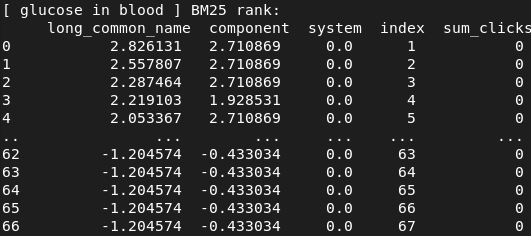
\includegraphics[width=0.6\textwidth]{include/bm25rank_glucoseBlood.png}
		\caption{Resultado de aplicar el algoritmo BM25.}
	\end{figure}
	
	Cabe destacar que con el algoritmo BM25, la importancia de los contenidos del system se marca como $0$ en todos los casos. Esto se debe a que este campo contiene abreviaturas, representando por ejemplo la palabra \textit{blood} como \textit{Bld}, por lo que una búsqueda por palabra exacta no obtiene ningún resultado.\\
	
	Como se indica en el articulo \cite{articulo-clase}, la información relativa al clickthrough data se codifica como tripletas, donde cada búsqueda (query) se relaciona con los resultados obtenidos con el algoritmo de búsqueda, y el número de clicks realizados sobre cada uno de ellos.
	
	
	El dataset apropiado para aplicar el algoritmo SVM rank, tiene un formato específico. En este caso, la consulta "glucose in blood" se representa como se indica en la figura 3, donde el primer campo indica el número de clicks del link, el segundo campo contiene un identificador de la consulta y los otros tres campos contienen el resultado del BM25 para cada uno de los campos estudiados.
	
	\begin{figure}[H]
		\centering
		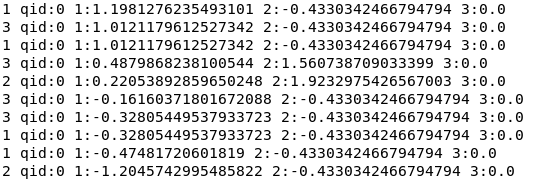
\includegraphics[width=0.6\textwidth]{include/SVMinput_glucoseBlood.png}
		\caption{Resultado de aplicar el algoritmo BM25.}
	\end{figure}
	
	De esta manera, se pudo generar un dataset con las tripletas habituales para este tipo de datos. Esta información se guardó en un segundo fichero, separando el dataset en datos de entrenamiento (\texttt{train.dat}) y datos de evaluación (\texttt{test.dat}).
	
	Debido a la cantidad de datos con los que se trabaja, los dataset generados son significativamente pequeños, por lo que este proyecto se debe tomar como una prueba de concepto, y no una evaluación completa del algoritmo.
	
	\subsection{Implementación}
	
	La implementación realizada se puede observar en la carpeta adjunta \texttt{code}, que contiene los ficheros de código necesarios, así como los ficheros de entrada del algoritmo en la carpeta \texttt{code/loinc\_dataset} y los resultados de la ejecución en la carpeta \texttt{code/result}.
	
	Para la implementación, la información se separó en dos dataset. El dataset \textit{train}, que contiene las primeras 50 filas, se utilizó para entrenar el algoritmo, mientras que el conjunto \textit{test} se utilizó para mejorar la búsqueda y así poder evaluar el algoritmo.
	
	La implementación realizada sigue el siguiente esquema
	
	\begin{figure}[H]
		\centering
		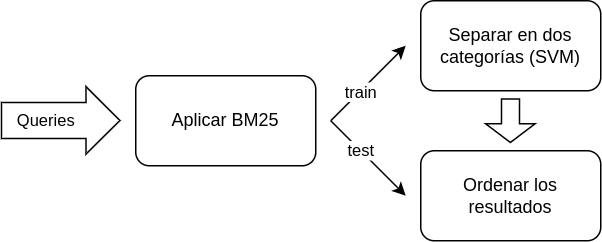
\includegraphics[width=0.6\textwidth]{include/esquema_implementacion.png}
		\caption{Esquema de la implementación}
	\end{figure}
	
	Veamos como se aplica esta implementación a la query \textit{"glucose in blood"}, glucosa en sangre, sobre el dataset proporcionado. 
	
	En primer lugar, 

	

	A continuación, utilizando la transformada pairwise y el modelo SVC linear, convertimos nuestro problema de búsqueda en un problema de clasificación bidimensional, teniendo en cuenta los clicks de los usuarios y el resultado de la búsqueda anterior. 
	
	Por último, ordenamos los resultados del dataset \texttt{test}, y generamos unas gráficas que nos permitan visualizar los resultados.
	
	\subsection{Testeo y resultados}
	
	
	
	\section{Conclusiones}
	

	%\section*{Bibliografía}
	%\addcontentsline{toc}{section}{Bibliografía}
	\bibliography{include/references}
	\bibliographystyle{IEEEtran}
	
	
\end{document}